This section first presents a background on component models and particularly on the Low Level Components. This background is needed to understand the second part of the section which gives an overview of the overall Multi-Stencil Framework (MSF).

%----------------------------------------
\subsection{Background on component models}
%----------------------------------------
Component-based software engineering (CBSE) is a domain of software engineering~\cite{Szyperski:2002:CSB:515228} which aims at improving code re-use, separations of concerns, and thus maintainability.
A component-based application is made of a set of component instances linked together, this is also called a component \emph{assembly}.
A component is a black box that implements an independent functionality of the application, and which interacts with its environment only through well defined interfaces: its ports.
For example, a port can specify services provided or required by the component.
With respect to high performance computing, some works have also shown
that component models can achieve the needed level of performance and
scalability while also helping in application portability~\cite{Bernholdt01052006, bigot:inria-00388508, UCHPC2015}.

Many component models exist, each of them with its own specificities.
Well known component models include, for example, the CORBA Component Model (CCM)~\cite{corba:omg06}, and the Grid Component Model (GCM)~\cite{Baude} for distributed computing, while the Common Component Architecture (CCA)~\cite{Bernholdt01052006}, and Low Level Components (\llc)~\cite{l2c} are HPC-oriented.
This work makes use of \llc for the experiments.

\llc~\cite{l2c} is a minimalist \texttt{C++} based HPC-oriented component model
where a component extends the concept of class.
The services offered by the components are specified trough $provide$ ports,
those used either by $use$ ports for a single service instance,
or $use-multiple$ ports for multiple services instances.
Services are specified as \texttt{C++} interfaces.
\llc also offers $MPI$ ports that enable components to share MPI communicators. Finally, 
components can also have attribute ports to be configured.
%
In this paper, and as illustrated in Figure~\ref{fig:ports}, a $provide$ port is represented by a white circle, a $use$ port by a black circle, a $use-multiple$ port by a black circle with a white $m$ in it. MPI port are connected with a black rectangle. A \llc-based application is a static \emph{assembly} of components instances and the connections between their ports.
Such an assembly is described in LAD, an XML dialect, and is managed by the \llc runtime system that minimize overheads by loading simple dynamic libraries. One can also notice that \llc can achieve performance if the granularity of components is high enough and attentively chosen by the user. The typical overhead of a \llc is a \texttt{C++} indirect virtual method invocation.

\begin{figure}[t]
\begin{center}
\subfloat[][\label{fig:2comp}]{
\begin{tikzpicture}[shorten >=1pt, node distance=2cm, on grid, auto]
   \node[component] (C) at (0,0) {$c_0$};
   \node[provide] (p) at (-1.5,0) {};
   \node[use] (u) at (1.5,0) {};
   \node[provide,right=1.5cm of u] (p1) {};
   \node[component,right=1.5cm of p1] (C1) {$c_1$};
   \node[use,right=1.5cm of C1] (um) {$m$};
 
  \path[-]
    (p) edge node {$p$} (C)
    (C.east) edge node {$u$} (u)
    (C1)  edge node {$v$} (um)
    (p1) edge node {$q$} (C1);
\end{tikzpicture}
}
\\
\subfloat[][\label{fig:ass}]{
\begin{tikzpicture}[shorten >=1pt, node distance=2cm, on grid, auto]
   \node[component] (C) at (0,0) {$c_0$};
   \node[provide] (p) at (-1.5,0) {};
   \node[use] (u) at (1.5,0) {};
   \node[provide,right=0.15 of u] (p2) {};
   \node[component,right=1.5 of p2] (C1) {$c_1$};
   \node[use,right=1.5 of C1] (um) {$m$};
 
  \path[-]
    (p) edge node {$p$} (C)
    (C) edge node {$u$} (u)
    (C1)  edge node {$v$} (um)
    (p2) edge node {$q$} (C1);
\end{tikzpicture}
}
\\
\subfloat[][\label{fig:mpi}]{
\begin{tikzpicture}[shorten >=1pt, node distance=2cm, on grid, auto]
   \node[component] (C) at (0,0) {$c_2$};
   \node[provide] (p) at (-1.5,0) {};
   \node[mpi] (u) at (1.5,0) {};
   \node[component,right=1.5 of u] (C1) {$c_3$};
 
  \path[-]
    (p) edge node {} (C)
    (C) edge node {} (u)
    (u) edge node {} (C1);
\end{tikzpicture}
}
\caption{Example of components and their ports representation. a) Component $c_0$ has a provide port ($p$) and a use port ($u$); Component $c_1$ has also a provide port ($q$) but also a use multiple port ($v$). b) A use port is connected to a (compatible) provide port. c) Component $c_2$ and $c_3$ shares an MPI communicator.}
\label{fig:ports}
\end{center}
\end{figure}

%----------------------------------------
\subsection{Multi-Stencil Framework overview}
%----------------------------------------
The Multi-Stencil Framework helps end-users to produce high performance parallel applications for the specific case of multi-stencils. The multi-stencil domain will be formally defined in the next section.
A multi-stencil program numerically solves PDEs using computations that can use neighborhood values around an element, also called a \emph{stencil} computation.

Figure~\ref{fig:msf} gives an overview of the Multi-Stencil Framework that is entirely detailed throughout this paper. It is composed of four distinct parts described hereafter.
As illustrated in Figure~\ref{fig:msf}, MSF targets two different kinds of end-users: the \emph{numerician}, in other words the mathematician, and the \emph{developer}. Most of the time numericians do have programming knowledge, however as it is not their core domain and because of a lack of time, development is often left to engineers according to numerician needs. MSF has the interesting particularity to propose a clear separation of concerns between these two end-users by distinguishing the description of the simulation from the implementation of numerical codes.

MSF also has the interesting capability to be more flexible than existing solutions thanks to a possibility for a third party to interact with the framework. This third party is a High Performance Computing (HPC) specialist as displayed in Figure~\ref{fig:msf}.

\begin{figure}[t]
\begin{center}
  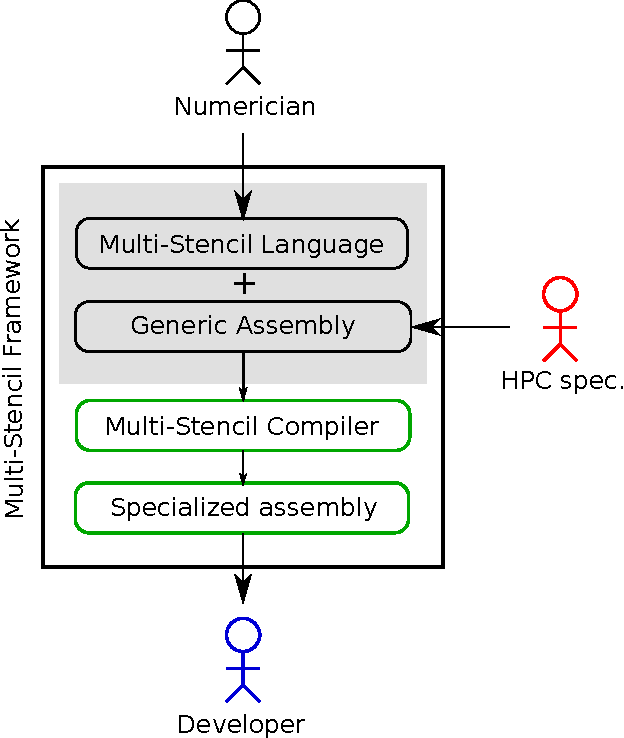
\includegraphics[width=.6\textwidth]{./images/msf.pdf}
  \caption{The Multi-Stencil Framework (MSF) is composed of the Multi-Stencil Language (MSL), the Generic Assembly (GA) and the Multi-Stencil Compiler (MSC) to produce a specialized assembly of components. The numerician, or mathematician uses MSL to describe its simulation. The developer will implement components responsible for numerical codes. A third party HPC specialist can interact with MSF to propose different version of HPC components.}
  \label{fig:msf}
\end{center}
\end{figure}

\paragraph{\textbf{Multi-Stencil Language}}
The Multi-Stencil Language, or MSL, is the domain specific language proposed by the framework for the numerician. It is a descriptive language, easy to use, without any concern about implementation details.
It fits the need of a mathematician to describe the simulation. The description written with MSL can be considered as an input of the framework. MSL is described in details in Section~\ref{sect:msl}. The language is built upon the formalism described in Section~\ref{sect:formalism}.

\paragraph{\textbf{Generic Assembly}}
In addition to the language MSL, used by the numerician to describe its simulation, MSF needs a Generic Assembly (GA) of a multi-stencil program as input. What is called a GA is a component assembly for which meta-types of components are represented and for which some parts need to be generated or specialized. A GA could be compared respectively to a template or a skeleton in object programming languages (such as C++) or functional languages. From this generic assembly will be built the final specialized assembly of the simulation where component types will be specified, and where parts of GA will be transformed. As well as MSL, this generic assembly is described in Section~\ref{sect:msl} and is built upon the meta-formalism described in Section~\ref{sect:formalism}.

\paragraph{\textbf{Multi-Stencil Compiler}}
The core of the framework is the Multi-Stencil Compiler, or MSC. It is responsible for transforming the generic assembly into the final parallel assembly which is specific to the simulation described by the numerician with MSL. MSC is described in Section~\ref{sect:parallelism}.

\paragraph{\textbf{Specialized assembly}}
Finally, the output of MSF is the component assembly generated by MSC. It is an instantiation and a transformation of the generic component assembly, by adding component types, transforming some part of the assembly, and by adding specific components generated by MSC. From this final component assembly which is specific to the simulation initially described with MSL, the developer will finally write components associated to numerical codes, or directly re-use existing components from other simulations. This final specialized component assembly is a parallel orchestration of the computations of the simulation initially described by the numerician. Finally, the specialized assembly produced by MSF is written in \llc.
